\documentclass[tikz, border=10pt]{standalone}
\usetikzlibrary{positioning}
\begin{document}
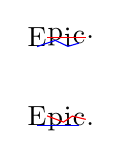
\begin{tikzpicture}[every node/.style = {inner sep=0pt}]
    \node (E) {E};
    \node (p) [right = 0pt of E] {p};
    \node (i) [right = 0pt of p] {i};
    \node (c) [right = 0pt of i] {c};
    \node (.) [right = 0pt of c] {.};
    \draw[red] (E.east) -- (p.east) -- (i.east) -- (c.east);
    \draw[blue] (E.base) -- (p.base) -- (i.base) -- (c.base);
    \node (E1) at (0, -1) {E};
    \node (p1) [base right = 0pt of E1] {p};
    \node (i1) [base right = 0pt of p1] {i};
    \node (c1) [base right = 0pt of i1] {c};
    \node (.1) [base right = 0pt of c1] {.};
    \draw[red] (E1.east) -- (p1.east) -- (i1.east) -- (c1.east);
    \draw[blue] (E1.base) -- (p1.base) -- (i1.base) -- (c1.base);
\end{tikzpicture}
\end{document}